\subsection{Electronic chain linearity}

In order to prepare the data acquistion system, the entire electronical chain
was tested beforehand. In fact it is crucial that the response of each
electronic device used behaves linearly, as the information about the energy
of the incident particle must be univocally extracted at the end of the chain.

\begin{figure}[h]
  \centering
  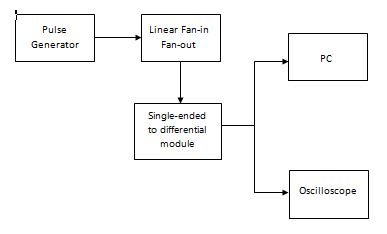
\includegraphics[scale=.5]{img/electronic_chain_diagram.JPG}
  \caption{The electronic chain}
  \label{chain}
\end{figure}

The setup used is shown in Fig.~\ref{chain}. The output of a pulse generator is fed into a Fan-in Fan-out which reproduces the same signal for 12 channels, this signals are given in input to a single-ended to differential amplifier custom board, in order to do this a cable was made.
The output of the board as seen from the oscilloscope is shown in Fig.~\ref{osc}.




From the board the signal is given to a 100 MHz 14-bit resolution digitizer throught a MDR-26 connector
At the signal is the applied, with an FPGA, a trapezoidal filter with its charateristics \emph{risetime} and \emph{flat top} width parameters, this step is crucial because because the height of the peak from the differential amplifier board will be directly proportional to the energy of the incident particle in the detector.
The height trapezoidal filter with the right parameters then gives the information on the intensity of the peak available for longer time.




\subsection{Testing the TRACE detector}

To test the PROTO Trace detector, it was put in a vacuum chamber, with a $\alpha$-ray source.